\section{系统实现}

\subsection{前端实现}

本系统的前端采用现代化的Web开发技术栈,基于Next.js 14框架构建.


如前端项目的组件关系图\ref{fig:front_end_structure}所示,系统采用了基于Next.js的分层设计,从配置层(config.ts、globals.css、fonts.ts)到导航布局(layout.tsx)再到具体的功能页面(MapPage、FilterPage、OverviewPage)。每个功能页面都对应特定的数据可视化组件(MapPlot、FilterPlot、OverviewPlot),这些组件分别使用了不同的可视化库(Plotly.js Map、NextUI组件、Plotly.js Charts和Dashboard)来实现地图展示、数据筛选和统计概览等功能。整个前端架构通过统一的API调用(salary-distribution、filter-data、overview-stats)与后端进行数据交互,实现了清晰的数据流动和模块化的功能划分。

\begin{figure}[htbp]
    \centering
    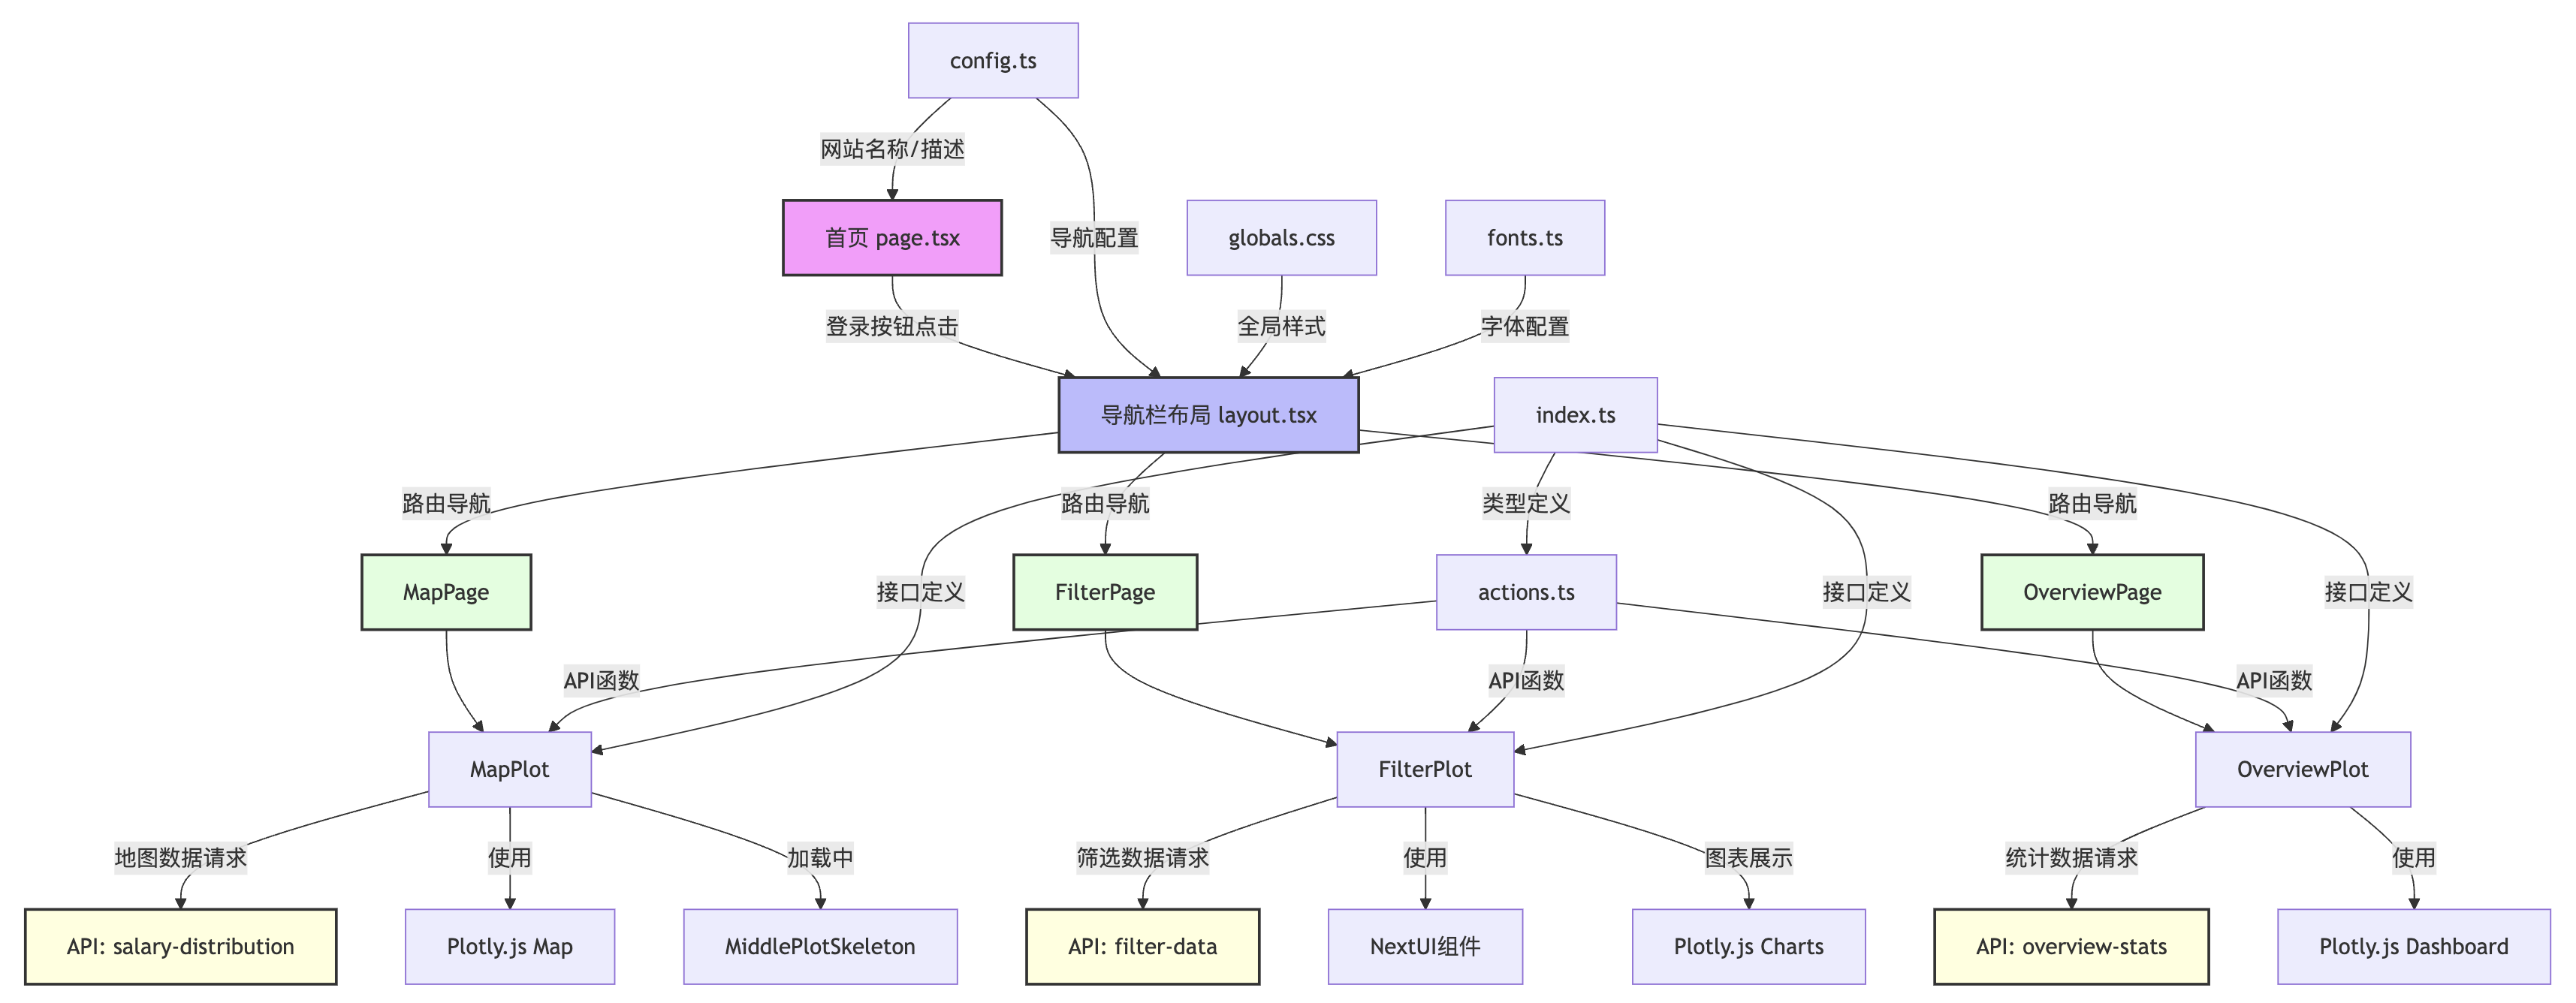
\includegraphics[width=1.0\textwidth]{figures/前端项目结构图.png}
    \caption{前端项目结构图}
    \label{fig:front_end_structure}
\end{figure}

如前端数据流图\ref{fig:front_end_data_flow}所示,系统采用了基于React Hooks的状态管理模式,从用户交互(用户点击、用户输入、用户选择)开始,通过useState和useEffect等钩子函数管理状态和副作用。数据流经过actions.ts进行统一的动作处理,然后通过fetch请求调用后端API。获取的数据经过数据解析和TypeScript类型转换后,最终通过Plotly.js或NextUI组件进行可视化展示,同时系统还实现了错误处理和加载状态显示,形成了一个完整的前端数据处理闭环。这种设计保证了数据流的单向性和可预测性,提高了应用的可维护性和性能。


\begin{figure}[htbp]
    \centering
    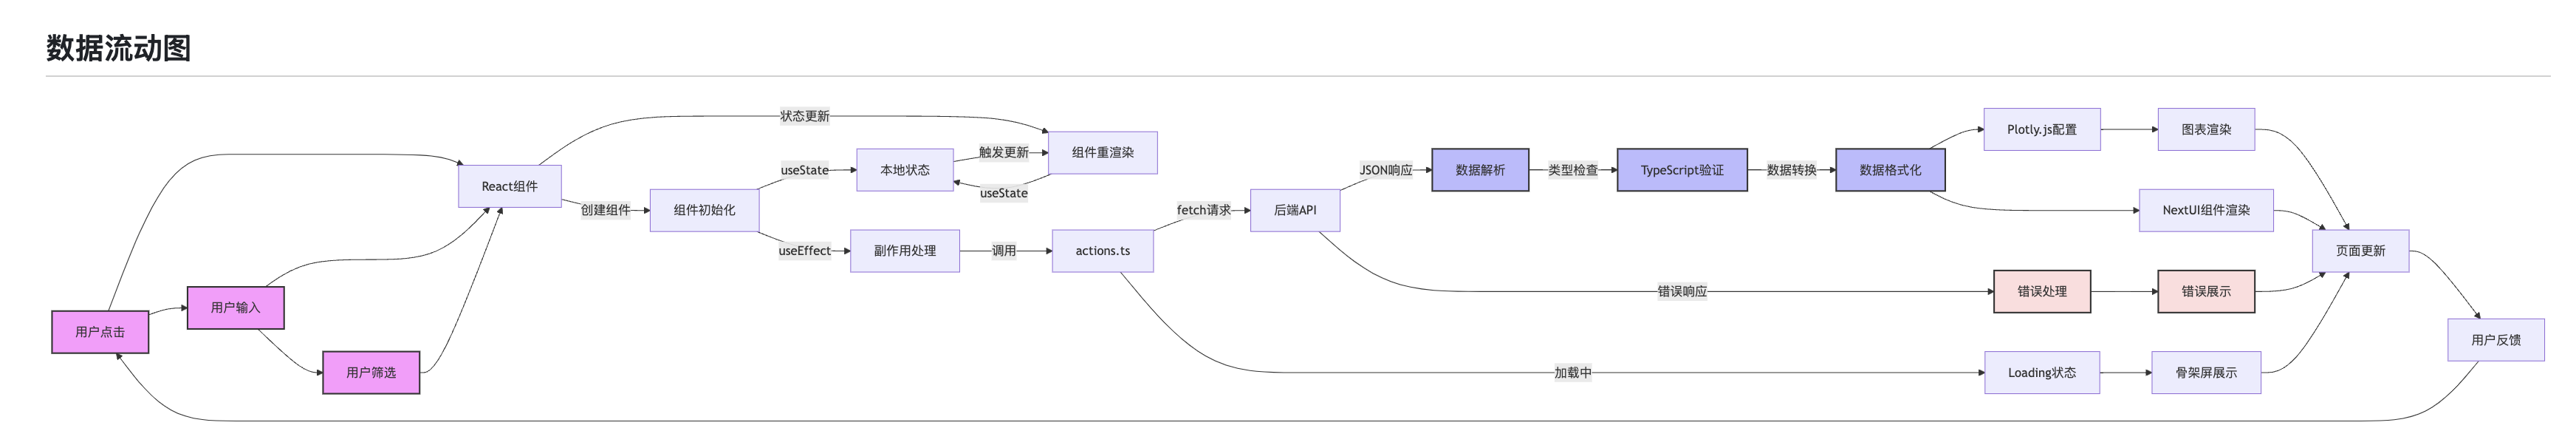
\includegraphics[width=1.0\textwidth]{figures/前端数据流图.png}
    \caption{前端数据流图}
    \label{fig:front_end_data_flow}
\end{figure}




\subsubsection{项目结构}
前端项目采用标准的Next.js项目结构,主要包括:
\begin{itemize}
    \item \texttt{app/}: 包含页面组件和路由配置
    \item \texttt{components/}: 可复用的UI组件
    \item \texttt{styles/}: 全局样式和主题配置
    \item \texttt{lib/}: 工具函数和API调用封装
    \item \texttt{public/}: 静态资源文件
\end{itemize}

\subsubsection{技术栈}
\begin{itemize}
    \item \textbf{核心框架}:Next.js 14,提供服务端渲染和路由管理
    \item \textbf{UI组件库}:NextUI v2,提供现代化的UI组件
    \item \textbf{样式管理}:Tailwind CSS,实现响应式设计
    \item \textbf{状态管理}:React Hooks,管理组件状态
    \item \textbf{数据可视化}:Echarts,实现各类图表展示
\end{itemize}

\subsubsection{功能实现}
前端实现了以下主要功能模块:
\begin{itemize}
    \item \textbf{数据展示}:
    \begin{itemize}
        \item 职位列表展示,支持分页和筛选
        \item 公司信息展示,包括详细信息和地理位置
        \item 数据统计图表,包括薪资分布、职位分布等
    \end{itemize}
    
    \item \textbf{数据分析}:
    \begin{itemize}
        \item 薪资分析模块,支持多维度对比
        \item 地理分布热力图,展示职位地理分布
        \item 行业趋势分析,展示行业发展趋势
    \end{itemize}
    
    \item \textbf{用户交互}:
    \begin{itemize}
        \item 响应式设计,适配不同设备
        \item 数据筛选和排序功能
        \item 图表交互和数据钻取
    \end{itemize}
\end{itemize}

\subsection{后端实现}

后端系统基于FastAPI框架开发,采用异步编程模式,主要实现包括:

\subsubsection{项目结构}
后端采用模块化的项目结构:
\begin{itemize}
    \item \texttt{app/}: 主应用目录
    \begin{itemize}
        \item \texttt{api/}: API路由和接口定义
        \item \texttt{crud/}: 数据库操作封装
        \item \texttt{db/}: 数据库模型和配置
        \item \texttt{core/}: 核心功能和配置
        \item \texttt{scrapers/}: 数据采集模块
    \end{itemize}
\end{itemize}

\subsubsection{核心功能实现}
\begin{itemize}
    \item \textbf{数据库连接}:
    \begin{itemize}
        \item 使用SQLAlchemy异步ORM
        \item 实现数据库连接池管理
        \item 支持事务和并发控制
    \end{itemize}
    
    \item \textbf{数据处理}:
    \begin{itemize}
        \item 实现数据清洗和转换逻辑
        \item 支持批量数据处理
        \item 实现数据验证和错误处理
    \end{itemize}
    
    \item \textbf{API服务}:
    \begin{itemize}
        \item 实现RESTful API接口
        \item 支持数据分页和过滤
        \item 实现缓存和性能优化
    \end{itemize}
\end{itemize}

\subsubsection{性能优化}
系统在实现过程中采取了多项性能优化措施:
\begin{itemize}
    \item \textbf{数据库优化}:
    \begin{itemize}
        \item 使用物化视图加速查询
        \item 建立合适的索引
        \item 实现查询缓存
    \end{itemize}
    
    \item \textbf{并发处理}:
    \begin{itemize}
        \item 采用异步IO处理请求
        \item 实现任务队列管理
        \item 优化并发连接处理
    \end{itemize}
\end{itemize}

